\documentclass[conference]{IEEEtran}

\usepackage{algorithmic}
\usepackage{amsfonts, amsmath, amsthm}
\usepackage{array}
\usepackage{bm}
\usepackage{booktabs}
\usepackage{caption}
\usepackage{cite}
\usepackage{fullpage}
\usepackage{gensymb}
\usepackage{geometry}
\usepackage{graphicx}
\usepackage{listings}
\usepackage{mathtools}
\usepackage{pifont}
\usepackage{textcomp}
\usepackage{tikz}
\usepackage{tkz-graph}
\usepackage{verbatim}
\usepackage{xcolor}

\usetikzlibrary{shapes.geometric}

\def\BibTeX{{\rm B\kern-.05em{\sc i\kern-.025em b}\kern-.08em
    T\kern-.1667em\lower.7ex\hbox{E}\kern-.125emX}}

\newcolumntype{L}{>{$}l<{$}} % math-mode version of "l" column type

\makeatletter
\newcommand\mathboxed[1]{%
    \mathpalette\@mathboxed{#1}%
}
\newcommand\@mathboxed[2]{%
    \tikz[baseline=(math.base),outer sep=auto]{\node[draw,rectangle,inner
    sep=2.8pt]
    (math) {$#1#2$};
    \path (math.north)--++(0,1pt);
    \path (math.south)--++(0,-1pt);}%
}
\makeatother

\begin{document}
\title{%
  CENG435 Term Project: Part One \\
  \large End-to-end delay calculation with network emulation delays}

\author{
    \IEEEauthorblockN{Narmin Aliyeva}
    \IEEEauthorblockA{}
\and
    \IEEEauthorblockN{Berk Ozbalci}
    \IEEEauthorblockA{}
}

\maketitle

\section{Introduction}
The experiment consists of two parts. In the first part, we measured the RTT\footnote{round-trip time}
between each neighboring node in a network. We determined the link costs of each link using the RTT
measurements, and found the shortest path between the source node and the destination node using
Dijkstra's algorithm. In the second part, we applied different levels of delays on these nodes for
three separate experiments, and measured the end-to-end delay between the source node and destination
node by comparing timestamps. Time synchronization was accomplished using NTP (RFC 5905).

\section{Design and Implementation}
We created two sets of scripts, one for network discovery and one for running the end-to-end delay
experiment. Both are written in Python 3.6.5, which were the version running on the GENI-allocated
machines at the time of starting the assignment. In addition, both scripts are heavily supported by
shell scripts in order to facilitate setting up nodes, links and retrieving the experiment results.


\subsubsection{Discovery Scripts}
The discovery script creates a \textit{messaging pair} at each node, for each of its
neighboring nodes. The messaging pair is a pair of UDP server and UDP client, and each of them
run in a separate thread. This means that for a node having three neighbors, it will have six
threads, three of them which are UDP servers, and the remaining UDP clients.

The messaging protocol is very straightforward: each message contains a \textit{sender ID}, which is
a unique identifier of the node that the message originates from; and an \textit{index}, which is the
sequence index at which the UDP client has sent the message.

The sender ID is used to decide whether an incoming message originates from the same messaging pair,
i.e. if the sender ID is same as the current node's sender ID, then it's a round-trip and we must
calculate RTT based on this message; otherwise, it originates from another node and therefore it
must be echoed back.

In our scheme, every node constructs a messaging pair with all of its neighbors. Therefore, a total
of 16 link costs have been measured. For each measurement, a total of 1,000 messages were sent,
and the results were averaged.

\subsubsection{Experiment Scripts}
The experiment script takes a routing information file as input, which is a simple linked list of
nodes that the end-to-end delay experiment will be conducted over. For example,

\begin{lstlisting}
["s", "r1", "r2", "r3"]
\end{lstlisting}

will set up sockets at each node in the following fashion:

\begin{itemize}
    \item \textbf{s} will send messages to \textbf{r1}
    \item \textbf{r1} echoes all messages to \textbf{r2}
    \item \textbf{r2} echoes all messages to \textbf{r3}
    \item \textbf{r3} calculates the end-to-end delay.
\end{itemize}

When the experiment script is run with the above routing input at node \textbf{r2}, it will find
that its name does not appear on the routing list, and therefore exits immediately.

The experiment scripts use a different message structure from the measurement scripts. The only
content is the UNIX timestamp with millisecond precision, represented as a floating point number.
When this message is received at the final node, the receiver node calculates the timestamp and
computes the difference between the received message's timestamp and its own timestamp. This
difference is the \textit{end-to-end delay}.

For this scheme to work, both the initial node and the final node must be time-synchronized. We
accomplished this by using an external NTP server:

\begin{lstlisting}
# ntpdate 0.tr.pool.ntp.org
\end{lstlisting}

\subsubsection{Common Implementation Details}
\begin{itemize}
    \item Network emulation delay is achieved by using the \textbf{tc} commands.
    \item All nodes receive the network topology in an adjacency list format, and compute their neighbors dynamically.
    \item In the discovery messages, both \textbf{sender\_id} and \textbf{index} are represented as integers.
    \item In the experiment messages, \textbf{timestamp} is IEEE 754 double-precision floating number.
    \item For both measurement and experimentation, we picked a base port (10000) and applied the following convention:
    \begin{itemize}
        \item Each server host listens to packages from a client host on port $B + C$, where $B$ is the base port, and $C$ is the sender ID of the client host.
    \end{itemize}
\end{itemize}

\section{Network Topology and RTTs}
The measurement script was ran on all nodes, but we have obtained the RTTs shown in Fig. \ref{fig:links}
from the inner nodes only (\textbf{r1}, \textbf{r2} and \textbf{r3}).

\begin{figure}
\centering
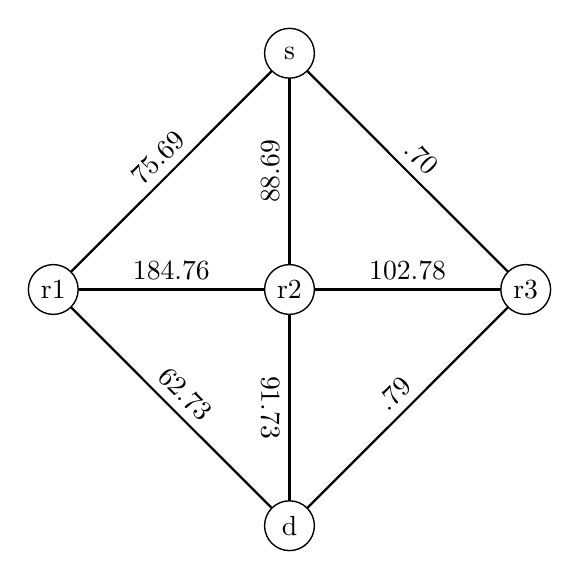
\begin{tikzpicture}
  \Vertex[x=0,y=6]{s}
  \Vertex[x=-3,y=3]{r1}
  \Vertex[x=0,y=3]{r2}
  \Vertex[x=3,y=3]{r3}
  \Vertex[x=0,y=0]{d}
  \tikzstyle{LabelStyle}=[sloped]
  \tikzstyle{EdgeStyle}=[]
  \Edge[label=$75.69$,labelstyle={pos=0.5,above}](r1)(s)
  \Edge[label=$184.76$,labelstyle={pos=0.5,above}](r1)(r2)
  \Edge[label=$62.73$,labelstyle={pos=0.5,above}](r1)(d)
  \Edge[label=$88.69$,labelstyle={pos=0.5,above}](r2)(s)
  \Edge[label=$91.73$,labelstyle={pos=0.5,below}](r2)(d)
  \Edge[label=$.70$,labelstyle={pos=0.5,above}](r3)(s)
  \Edge[label=$102.78$,labelstyle={pos=0.5,above}](r3)(r2)
  \Edge[label=$.79$,labelstyle={pos=0.5,above}](r3)(d)
\end{tikzpicture}
\caption{Network topology and link costs (ms)}
\label{fig:links}
\end{figure}

\section{Determining the Shortest Path using Dijkstra's Algorithm}

The following table is constructed for calculating the shortest path from \textbf{s} to
any other node in the network. The costs are expressed as RTTs in milliseconds.

\begin{table}[h]
\centering
\renewcommand{\arraystretch}{1.4}
\begin{tabular}{|L|L|L|L|L|L|}
\hline
\text{node} & s & r1 & r2 & r3 & d \\
\hline
s & \mathboxed{0_{s}} & 75.69_{s} & 88.69_{s} & .70_{s} & \infty \\
\hline
r3 & & 75.69_{s} & 88.69_{s} & \mathboxed{.70_{s}} & 1.49_{r3} \\
\hline
d & & 64.23_{d} & 88.69_{s} & & \mathboxed{1.49_{r3}} \\
\hline
r1 & & \mathboxed{64.23_{d}} & 88.69_{s} & & \\
\hline
r2 & & & \mathboxed{88.69_{s}} & & \\
\hline
\end{tabular}
\end{table}

First, we start by exploring the node \textbf{s}. It has three direct neighbors, and we add the
costs of those links to the first row. For any other node, the weight is set to infinity. We then
proceed to the next step by choosing to follow the link with the lowest cost, arriving at
\textbf{r3}. For any node reachable from \textbf{r3}, we check whether the cost from \textbf{r3} is
smaller than the minimum cost that is already found (if it exists). If it is smaller, we take that
step, adding that link's cost to the prior calculation in order to find the total cost of reaching
the node from the starting node. Otherwise, we keep the previous result as is.

The subscripts at each table cell indicate the node that was used in order to reach at the number
shown in the table cell. That is, $.70_{s}$ indicates that the node in question can be reached
from \textbf{s}, and the total cost of doing so is $0.70$.

As can be seen from the table, the shortest path between \textbf{s} and \textbf{d} is

\begin{lstlisting}
["s", "r3", "d"]
\end{lstlisting}

We believe that this is a natural result, since there is no preconfigured network emulation delay
on the links from \textbf{s} to \textbf{r3}, and \textbf{r3} to \textbf{d}.\footnote{Unlike the
nodes \textbf{r1} and \textbf{r2}, which have network emulation delays associated with all of
their outgoing links, which are defined in the assignment bundled scripts,
\textbf{configureR1.sh}, \textbf{configureR2.sh}.}

\section{The Effect of Network Emulation Delay on End-to-End Delay}

We conducted three experiments with varying levels of network emulation delay.

\begin{itemize}
    \item \textbf{Experiment I.} Delay of 20ms $\pm$ 5ms
    \item \textbf{Experiment II.} Delay of 40ms $\pm$ 5ms
    \item \textbf{Experiment III.} Delay of 50ms $\pm$ 5ms
\end{itemize}

All of the above experiments also use normal distribution to vary the amount of delay impacted to
the adapters.

To obtain a more accurate result, we've conducted the end-to-end delay transmission for 100 messages
at each experiment. In order to construct a 95\% confidence interval, we needed at least 30 samples,
but since we've automated most of the script fairly well, we confidently increased the test size.

The experimental data is provided in the below table. CI denotes "Confidence Interval".

\begin{table}[h]
    \centering
\renewcommand{\arraystretch}{2.5}
    \begin{tabular}{|c|c|c|c|}
\hline
              & Exp. I & Exp. II & Exp. III \\
\hline
        Mean  & 38.74  & 81.95   & 99.45 \\
\hline
        CI min & 37.44 & 80.57 & 97.95 \\
\hline
        CI max & 40.02 & 83.31 & 100.95 \\
\hline
    \end{tabular}
    \caption{End-to-end delay mean and confidence intervals}
    \label{table:data}
\end{table}

Initially we expected the mean end-to-end delay to be approximately twice of the network emulation
delay applied to each node, because there are only two links in the path and they both have the
same amount of delay associated with them.

Upon running the experiments, we have met our initial expectations with very close results.

\begin{figure}
    \center
    \includegraphics[width=\columnwidth]{images/chart}
    \caption{Network emulation delay vs.\ end-to-end delay}
    \label{fig:graph}
\end{figure}


\section{Further Implementation Details}
This section contains more specific implementation details on various parts of the project.

\subsection{The Nature of UDP: Ensuring the Right Number of Messages}
Since UDP does not guarantee that all packets that are sent will arrive at the destination host,
we didn't use a simple counter that attempts to send a message exactly $N$ times, where $N$ is the
size of the experiment currently running.

In the discovery part, each messaging pair maintains the number of packets that have successfully
returned from a round-trip. The clients keep on sending new messages until this number reaches $N$,
the experiment size. Since both the server and the client threads are reading and writing to this
variable, we used mutexes to prevent race conditions and ensure that no lack or excess of packets
occur while calculating the average RTT.

In the experiment part, we apply a similar logic to the final node, which causes all the packets
sent from the penultimate node to be dropped, thereby restricting the data set to the exact count
of samples requested.

\subsection{End-to-End Delay vs. Round-Trip Time}
Our computation of the end-to-end delay and round-trip time differs in their implementation detail.

RTTs are computed by taking the difference of the timestamps at each packet event (being sent or
received) at the same node. That is, if node A sends a packet to node B at time $t_0$, and node
B sends back the same message to node A at time $t_1$, the round-trip time will be $t_1 - t_0$.

But end-to-end delays are computed by taking the difference between timestamps at different nodes.
This means that, if node A sends a packet at its local time $t_0$, and node B receives that packet
at its local time $t'_1$, the end-to-end delay will be measured as

$$
t'_1 - t_0 + \delta_{s}
$$

where $\delta_{s}$ is the synchronization offset, which is the time difference between nodes A
and B. To produce a more accurate end-to-end delay measurement, $\delta_{s}$ must be as small as
possible. We used NTP as a synchronization protocol to reduce the time difference between nodes.

\end{document}
